\documentclass[border=4pt]{standalone}
\usepackage{amsmath,amssymb}
\usepackage{tikz}
\usetikzlibrary{patterns}
\begin{document}
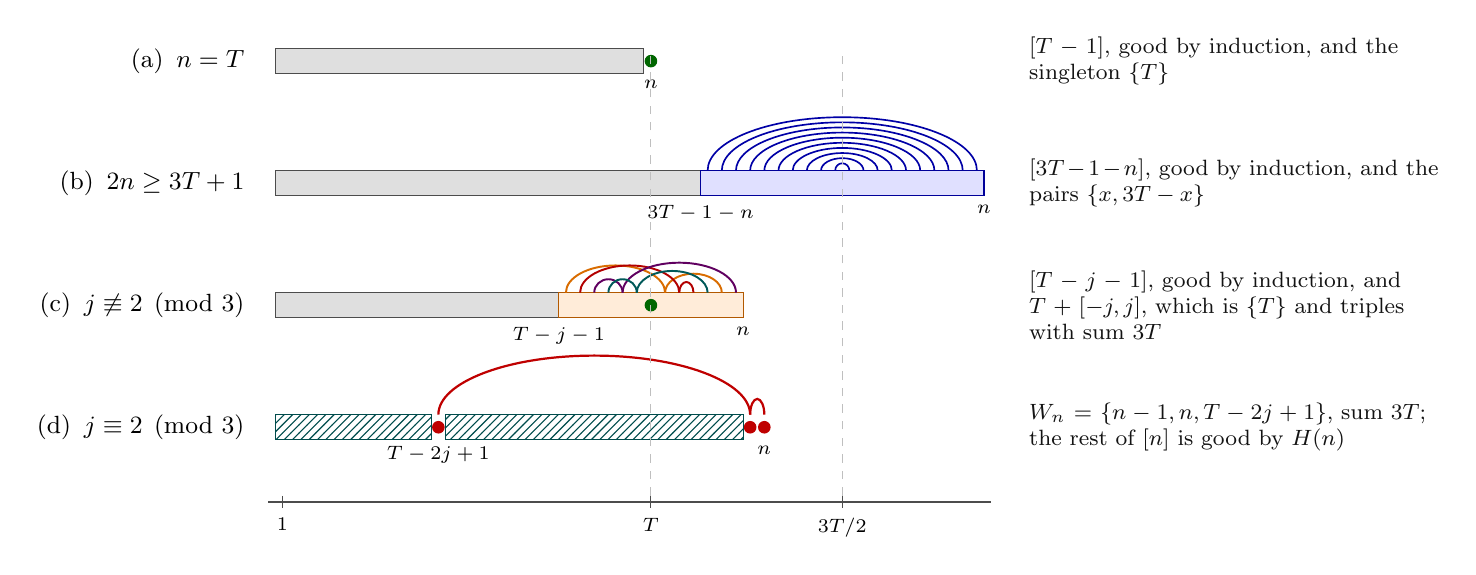
\begin{tikzpicture}[
  x=0.18cm, y=1cm,
  lab/.style={font=\small,anchor=east},
  note/.style={font=\footnotesize,gray!15!black,align=left,anchor=west,text width=5.2cm},
  old/.style={fill=gray!25,draw=gray!60!black,line width=0.4pt},
  pt/.style={circle,inner sep=0pt,minimum size=1.6mm}]
  \def\h{0.16}
  % (a) n = T = 27
  \begin{scope}[yshift=0cm]
    \node[lab] at (-1,0) {(a)\enspace $n=T$};
    \draw[old] (0.5,-\h) rectangle (26.5,\h);
    \node[pt,fill=green!40!black] at (27,0) {};
    \node[font=\scriptsize,anchor=north] at (27,-0.12) {$n$};
    \node[note] at (53,0) {$[T-1]$, good by induction, and the singleton $\{T\}$};
  \end{scope}
  % (b) n = 50, a = 3T-1-n = 30
  \begin{scope}[yshift=-1.55cm]
    \node[lab] at (-1,0) {(b)\enspace $2n\ge 3T+1$};
    \draw[old] (0.5,-\h) rectangle (30.5,\h);
    \fill[blue!12] (30.5,-\h) rectangle (50.5,\h);
    \draw[blue!60!black,line width=0.4pt] (30.5,-\h) rectangle (50.5,\h);
    \foreach \x in {31,...,40} {
      \pgfmathsetmacro{\r}{(81-2*\x)/2}
      \draw[blue!65!black,line width=0.6pt] (\x,\h) arc[start angle=180,end angle=0,x radius=\r,y radius={0.065*\r+0.06}];
    }
    \node[font=\scriptsize,anchor=north] at (50.5,-\h) {$n$};
    \node[font=\scriptsize,anchor=north] at (30.5,-\h) {$3T-1-n$};
    \node[note] at (53,0) {$[3T-1-n]$, good by induction, and the pairs $\{x,3T-x\}$};
  \end{scope}
  % (c) n = 33, j = 6
  \begin{scope}[yshift=-3.1cm]
    \node[lab] at (-1,0) {(c)\enspace $j\not\equiv 2\pmod 3$};
    \draw[old] (0.5,-\h) rectangle (20.5,\h);
    \fill[orange!15] (20.5,-\h) rectangle (33.5,\h);
    \draw[orange!70!black,line width=0.4pt] (20.5,-\h) rectangle (33.5,\h);
    \foreach \a/\b/\c/\col in {21/28/32/orange!85!black, 22/29/30/red!70!black, 23/25/33/violet!75!black, 24/26/31/teal!70!black} {
      \pgfmathsetmacro{\ra}{(\b-\a)/2}
      \pgfmathsetmacro{\rb}{(\c-\b)/2}
      \draw[\col,line width=0.7pt] (\a,\h) arc[start angle=180,end angle=0,x radius=\ra,y radius={0.07*\ra+0.1}];
      \draw[\col,line width=0.7pt] (\b,\h) arc[start angle=180,end angle=0,x radius=\rb,y radius={0.07*\rb+0.1}];
    }
    \node[pt,fill=green!40!black] at (27,0) {};
    \node[font=\scriptsize,anchor=north] at (33.5,-\h) {$n$};
    \node[font=\scriptsize,anchor=north] at (20.5,-\h) {$T-j-1$};
    \node[note] at (53,0) {$[T-j-1]$, good by induction, and $T+[-j,j]$, which is $\{T\}$ and triples with sum $3T$};
  \end{scope}
  % (d) n = 35, j = 8
  \begin{scope}[yshift=-4.65cm]
    \node[lab] at (-1,0) {(d)\enspace $j\equiv 2\pmod 3$};
    \foreach \u/\v in {0.5/11.5, 12.5/33.5} {
      \fill[pattern=north east lines,pattern color=teal!60!black] (\u,-\h) rectangle (\v,\h);
      \draw[teal!60!black,line width=0.4pt] (\u,-\h) rectangle (\v,\h);
    }
    \foreach \x in {12,34,35} { \node[pt,fill=red!75!black] at (\x,0) {}; }
    \draw[red!75!black,line width=0.8pt] (12,\h) arc[start angle=180,end angle=0,x radius=11,y radius=0.75];
    \draw[red!75!black,line width=0.8pt] (34,\h) arc[start angle=180,end angle=0,x radius=0.5,y radius=0.2];
    \node[font=\scriptsize,anchor=north] at (35,-0.12) {$n$};
    \node[font=\scriptsize,anchor=north] at (12,-0.12) {$T-2j+1$};
    \node[note] at (53,0) {$W_n=\{n-1,n,T-2j+1\}$, sum $3T$; the rest of $[n]$ is good by $H(n)$};
  \end{scope}
  % axis
  \begin{scope}[yshift=-5.6cm]
    \draw[gray!60!black,line width=0.5pt] (0,0) -- (51,0);
    \foreach \x/\t in {1/1, 27/T, 40.5/{3T/2}} {
      \draw[gray!60!black] (\x,0.08) -- (\x,-0.08);
      \node[font=\scriptsize,anchor=north] at (\x,-0.08) {$\t$};
    }
    \draw[gray!50,dashed,line width=0.4pt] (27,0.08) -- (27,5.75);
    \draw[gray!50,dashed,line width=0.4pt] (40.5,0.08) -- (40.5,5.75);
  \end{scope}
\end{tikzpicture}
\end{document}
